% Compile with: xelatex main.tex (twice).
% Theme: metropolis (installed under /usr/share/texlive/texmf-dist/tex/latex/beamertheme-metropolis).
\documentclass[aspectratio=169,10pt]{beamer}

\usetheme{metropolis}
\metroset{numbering=fraction,progressbar=foot}

\usepackage{amsmath,amssymb}
\usepackage{braket}
\usepackage{physics}
\usepackage{tikz}
\usetikzlibrary{positioning,arrows.meta,decorations.pathreplacing,decorations.pathmorphing,fit,backgrounds}
\usepackage{booktabs}
\usepackage{xcolor}

\definecolor{e0col}{HTML}{1F77B4}
\definecolor{e1col}{HTML}{D62728}
\definecolor{midcol}{HTML}{6F42C1}

\title{Bell-State Preparation on a Two-Legged Ladder QPU}
\subtitle{Dynamic swap, and unitary GHZ-uncompute}
\date{2026 NCCU Applied Physics Challenge --- 14 May 2026}
\author{Victor Liu, Weison Lin, Aaron Liao}

\begin{document}

\maketitle

% ============================================================
% Slide 2 — The challenge
% ============================================================
\begin{frame}{The Challenge}
  \begin{columns}[T,onlytextwidth]
    \begin{column}{0.42\textwidth}
      \textbf{Goal.} Prepare a Bell state
      \[
        \ket{\Phi^+}_{e_0 e_1}
          = \tfrac{1}{\sqrt{2}}\bigl(\ket{00}+\ket{11}\bigr)
      \]
      between the two \emph{far-end} qubits of a two-legged ladder QPU,
      for any ladder length~$L$.
      \medskip

      \textbf{Constraints.}
      \begin{itemize}\setlength{\itemsep}{0.2em}
        \item Only nearest-neighbour gates (ladder edges).
        \item Top leg, bottom leg, rungs all allowed.
        \item Must scale to arbitrary $L$.
      \end{itemize}
    \end{column}
    \begin{column}{0.58\textwidth}
      \centering
      \begin{figure}
          \centering
          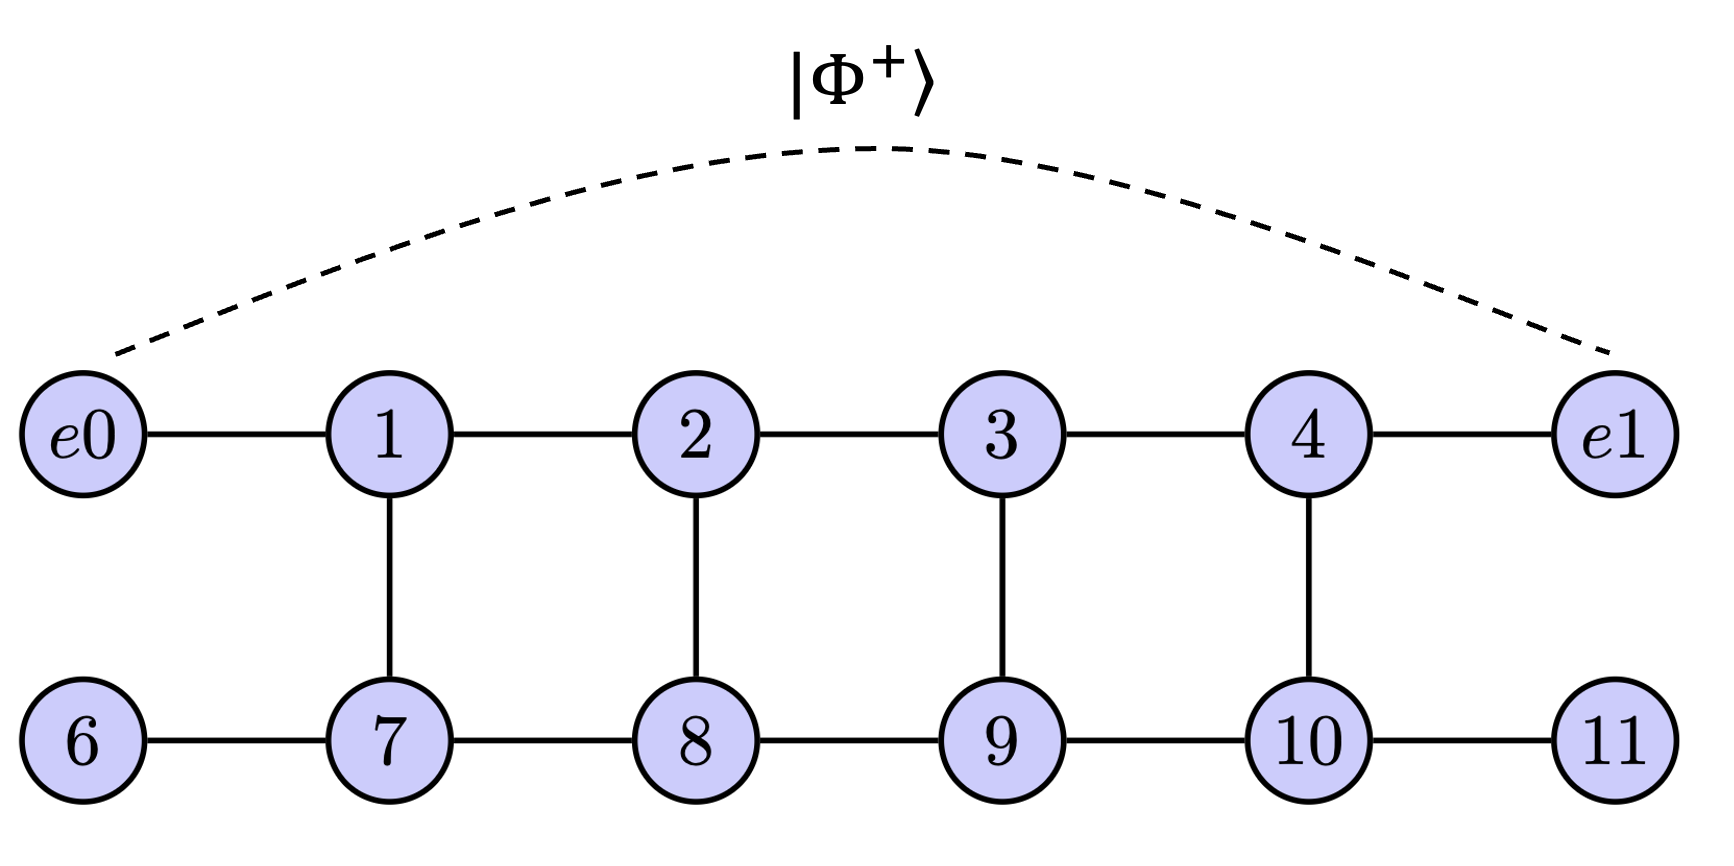
\includegraphics[width=0.9\linewidth]{figures/problem.png}
          \caption{The challenge example: $L=5$ (12 qubits).}
          \label{fig:placeholder}
      \end{figure}
      \vspace{0.4em}
    \end{column}
  \end{columns}
\end{frame}

% ============================================================
% Slide 3 — Protocol introduction
% ============================================================
\begin{frame}{Our Protocols}
  \begin{block}{1. Entanglement Swapping with Feed-Forward}\vspace{0.4em}
    \quad Uses alternating Bell pairs, Bell measurements on intermediate qubits, and a final classically controlled Pauli correction to deterministically entangle the endpoints.\\
    \vspace{0.4em}
    \textbf{Benefit:} Constant quantum depth independent of ladder length.
  \end{block}
  \pause
  \begin{block}{2. Middle-Out GHZ-Uncompute (MOGU)}\vspace{0.4em}
    \quad Builds a GHZ state from the middle of the top leg outward, then uncomputes the intermediate qubits to leave only the endpoints in a Bell state.\\
    \vspace{0.4em}
    \textbf{Benefit:} Measurement-free operation with optimal linear depth.
  \end{block}
\end{frame}

% ============================================================
% Slide 4 — Motivation 1: entanglement swapping
% ============================================================
\begin{frame}{Motivation 1: Entanglement swapping}
  \footnotesize
  Start with two Bell pairs $(0,1)$, $(2,3)$ — Bell-measure the middle pair $(1,3)$ —
  Pauli-correct $0$ or $3$ based on the outcome — $0,3$ end up in $\ket{\Phi^+}$ though they never interacted.

  \begin{center}
    \begin{figure}
        \centering
        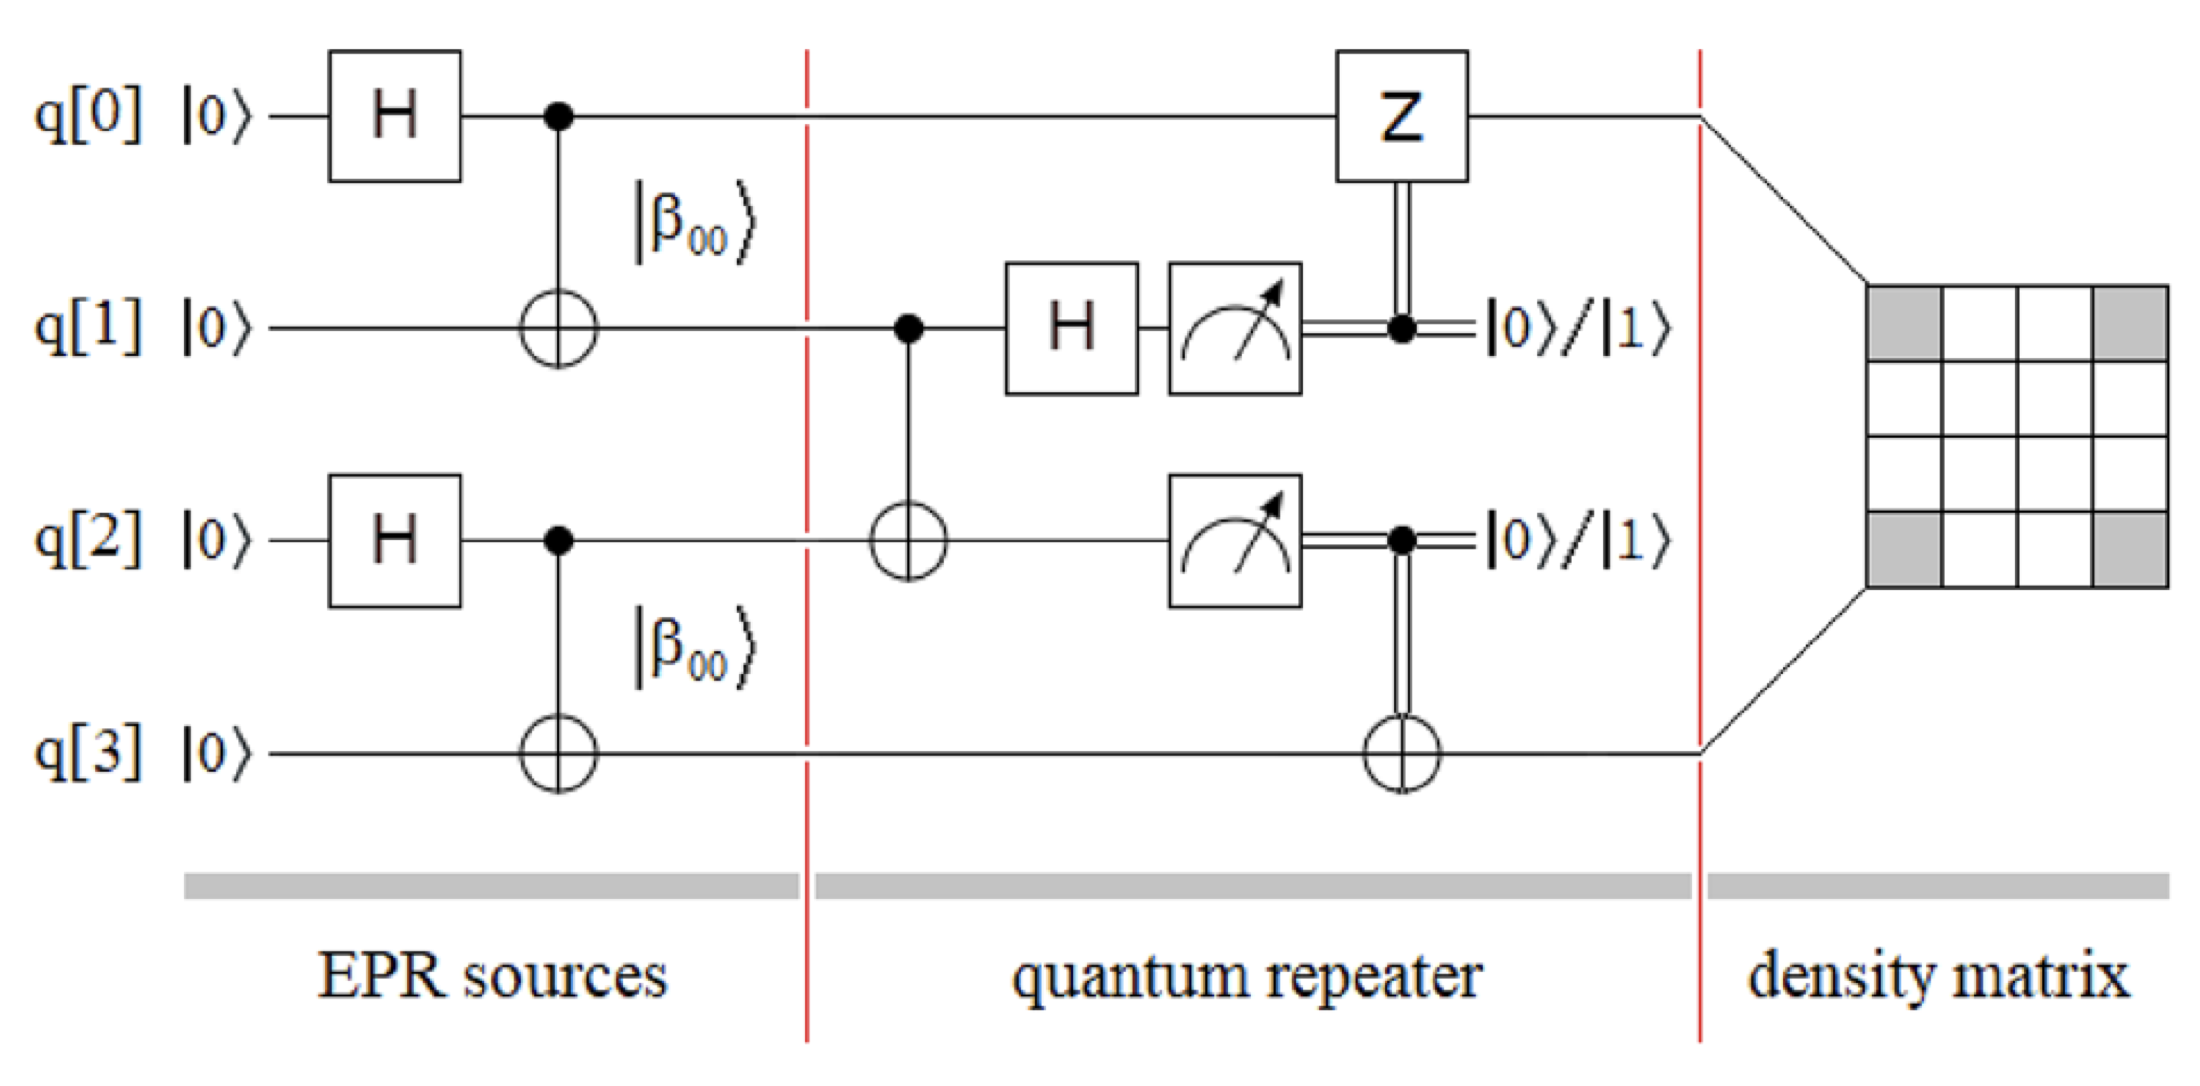
\includegraphics[width=0.5\linewidth]{figures/entanglement_swap.png}
        \caption{Quantum circuit for entanglement swapping}
        \label{fig:placeholder}
    \end{figure}
  \end{center}

  \scriptsize
  Mastriani, \textit{Sci. Rep.} 13, 21998 (2023)
\end{frame}

% ============================================================
% Slide 6 — Protocol I: overview circuit
% ============================================================
\begin{frame}{Protocol I — Entanglement-swap with feed-forward}
  \footnotesize
  \textbf{Three layers, $O(1)$ depth:} (1)~three Bell pairs on alternating
  links; (2)~two parallel Bell-measurements on the inner pairs;
  (3)~classically-controlled Pauli correction on $e_1$.
  \begin{center}
    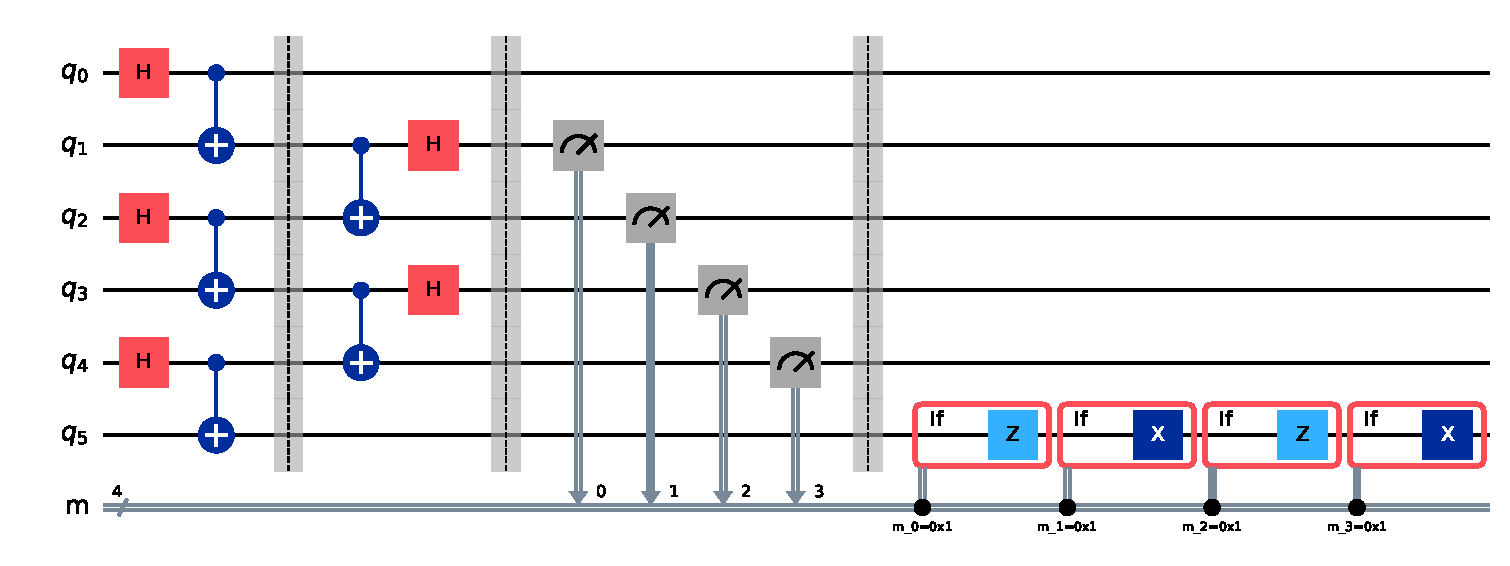
\includegraphics[width=0.95\textwidth]{figures/circuit_swap_L5.pdf}
  \end{center}
\end{frame}

% ============================================================
% Slide 7 — Protocol I: equations
% ============================================================
\begin{frame}{Protocol I — The Core Math: Stabilizer}
  We represent quantum state with stabilizer.\\
  The quantum state is the eigenstates of all stabilizer with +1 as eigenvalue.
  \pause
  
  \vspace{0.4em}
  
  Example 1: $\ket{\Phi^+}=\frac{\ket{00}+\ket{11}}{\sqrt{2}}$ can be represented by two stabilizer:
  \[
    \boxed{X_1X_2, \ Z_1Z_2}
  \]

  Example 2: $\ket{000000}$ can be represented by six stabilizer:
  \[
    \boxed{Z_1,\ Z_2,\ Z_3,\ Z_4,\ Z_5,\ Z_6}
  \]
  
\end{frame}

% ============================================================
% Slide 7 — Protocol I: equations
% ============================================================
\begin{frame}{Protocol I — The Core Math: Stabilizer transformation}
  The gate operation results in stabilizer transformation
  \pause
  
  \vspace{0.4em}
  
  1. Hadamard Transform
    \begin{align}
       &H_iX_iH_i=Z_i ,\ H_iZ_iH_i=X_i \\
        \Rightarrow &Z_i\longrightarrow X_i, \quad X_i\longrightarrow Z_i
    \end{align}

  \pause
  2. CNOT Transform
    \begin{align}
       &X_c\longrightarrow X_cX_t, \quad X_t\longrightarrow X_t\\
        &Z_c\longrightarrow Z_c, \quad Z_t\longrightarrow Z_cZ_t
    \end{align}
    \pause

    We used these rules to derive the Stabilizer for the final state.
\end{frame}

% ============================================================
% Slide 7 — Protocol I: equations
% ============================================================

\begin{frame}{Protocol I — The Core Math: Results}
  After the Bell-measurement layer, the residual stabilisers on $(e_0,e_1)$
  reduce to
  \[
    \tilde P_{XX} = (-1)^{m_1+m_3}\,X_{e_0}X_{e_1},
    \qquad
    \tilde P_{ZZ} = (-1)^{m_2+m_4}\,Z_{e_0}Z_{e_1}.
  \]
  \pause
  Feed-forward Pauli correction on $e_1$:
  \[
    \boxed{\;X^{\,m_2\oplus m_4}\;Z^{\,m_1\oplus m_3}\;}
  \]
  collapses both signs to $+1$, so every measurement branch deterministically
  prepares $\ket{\Phi^+}_{e_0 e_1}$.
  \pause
  \medskip
  \begin{block}{Generalisation}
    \begin{itemize}
      \item Even $N$: induction on Bell-pair count $\Rightarrow$ depth $\leq 7$
            for all $L$.
      \item Odd $N$: a single GHZ-3 link at the tail handles the parity obstruction.
    \end{itemize}
  \end{block}

  \footnotesize
  \textbf{Resources.} $N{+}1$ or $N{+}2$ two-qubit gates, $N$ measurements,
  constant depth.
\end{frame}

% ============================================================
% Slide 5 — Motivation B: GHZ-uncompute
% ============================================================
\begin{frame}{Motivation 2: GHZ-uncompute}
  \footnotesize
  \textbf{Idea.} If you cannot measure, build the entanglement everywhere
  and then carefully \emph{uncompute} what you don't want.
  \begin{enumerate}\setlength{\itemsep}{0.1em}
    \item Create GHZ state $\frac{1}{\sqrt 2}(\ket{0\cdots0}+\ket{1\cdots1})$ across the top leg.
    \item Reverse the fan-out from the centre outward
          $\Rightarrow$ interior qubits return to $\ket{0}$; only the endpoints stay entangled.
  \end{enumerate}

  \begin{center}
    \begin{figure}
        \centering
        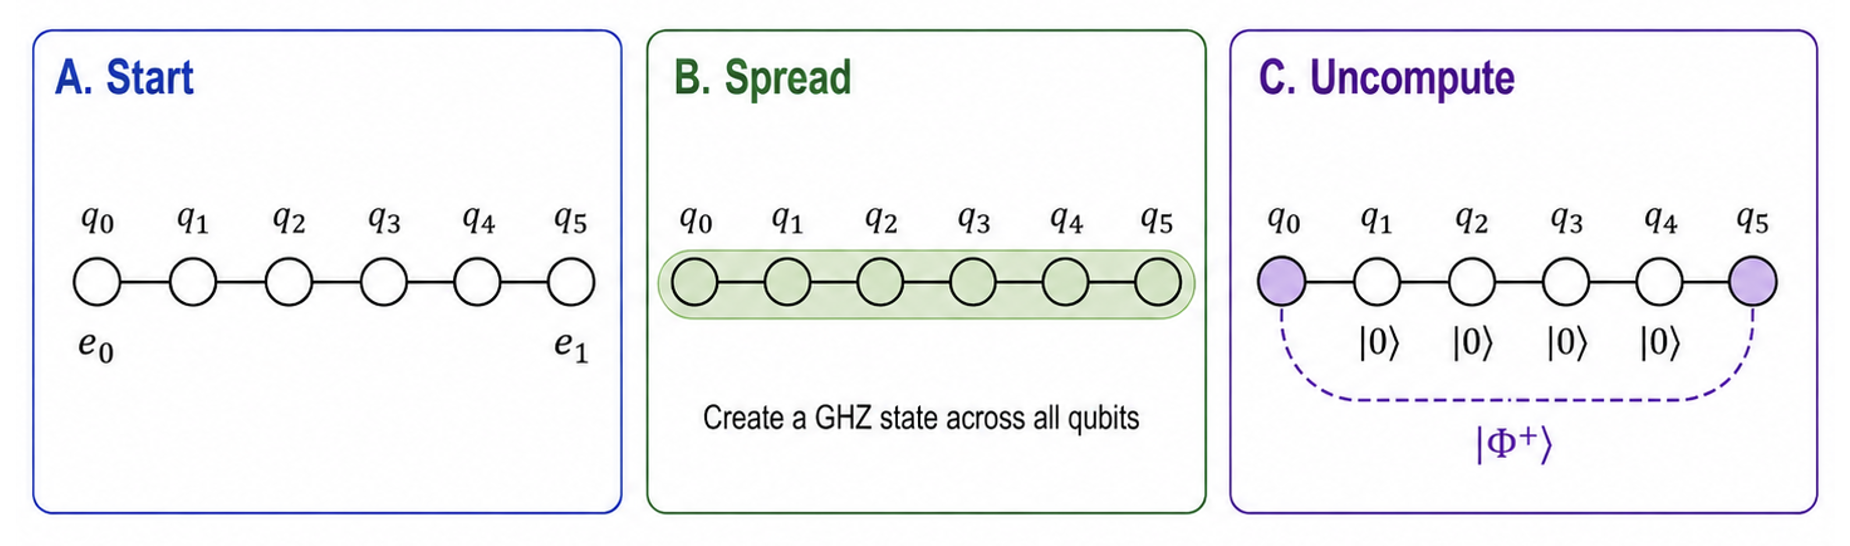
\includegraphics[width=0.7\linewidth]{figures/GHZ.png}
        \caption{Create GHZ state across all qubits and then disentangle the middle qubits.}
        \label{fig:placeholder}
    \end{figure}
  \end{center}
  \scriptsize
  In this way, there is \alert{zero measurements}. We call this
  \textbf{MOGU} = \emph{Middle-Out GHZ-Uncompute}.
\end{frame}

% ============================================================
% Slide 8 — Protocol II: overview circuit
% ============================================================
\begin{frame}{Protocol II — MOGU (measurement-free)}
  \footnotesize
  \textbf{Three phases:} (1)~$H$ on middle qubit $q_{\lfloor L/2 \rfloor}$;
  (2)~\alert{spread} CNOTs fan out from middle to ends;
  (3)~\alert{shrink} reverse-fan-out disentangles every interior qubit, centre outward.
  \begin{center}
    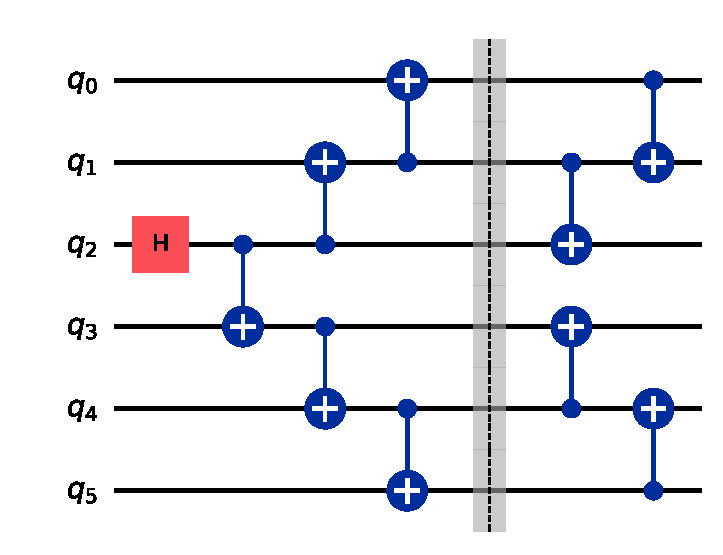
\includegraphics[height=0.62\textheight,keepaspectratio]{figures/circuit_mogu_L5.pdf}
  \end{center}
\end{frame}

% ============================================================
% Slide 9 — Protocol II: equations + parallel remark
% ============================================================
\begin{frame}{Protocol II — Core formulas}
  \textbf{Sequential schedule.}
  \[
    \text{depth} = L+2,\quad
    \text{2Q gates} = 2L-1,\quad
    \text{measurements} = 0.
  \]
  \pause
  \textbf{Stabiliser sketch.} After Phase~B the state is the standard $(L{+}1)$-qubit
  GHZ. Phase~C peels off each interior $Z_i$ generator, leaving
  \[
    \langle X_{e_0}X_{e_1},\; Z_{e_0}Z_{e_1},\; Z_1,\dots,Z_{L-1}\rangle
    \;=\; \text{stab}\bigl(\ket{\Phi^+}_{e_0 e_1}\otimes\ket{0}^{\otimes L-1}\bigr).
  \]
  \pause
  \textbf{Parallel schedule} (documentation-only, not in the verified code):
  if we interleave Phase~C with the still-in-flight Phase~B, the depth drops to
  \[
    d_{\parallel}(L) \;\approx\;
      \begin{cases}
        \min(L+2,\; \lceil L/2\rceil + 4) & L\ \text{even},\\
        \min(L+1,\; \lceil L/2\rceil + 3) & L\ \text{odd}.
      \end{cases}
  \]
  \footnotesize\emph{$\approx 2\times$ depth reduction at large $L$ — free constant-factor win.}
\end{frame}

% ============================================================
% Slide 10 — Benchmark scaling
% ============================================================
\begin{frame}{Benchmark: Resources vs $L$}
  \begin{center}
    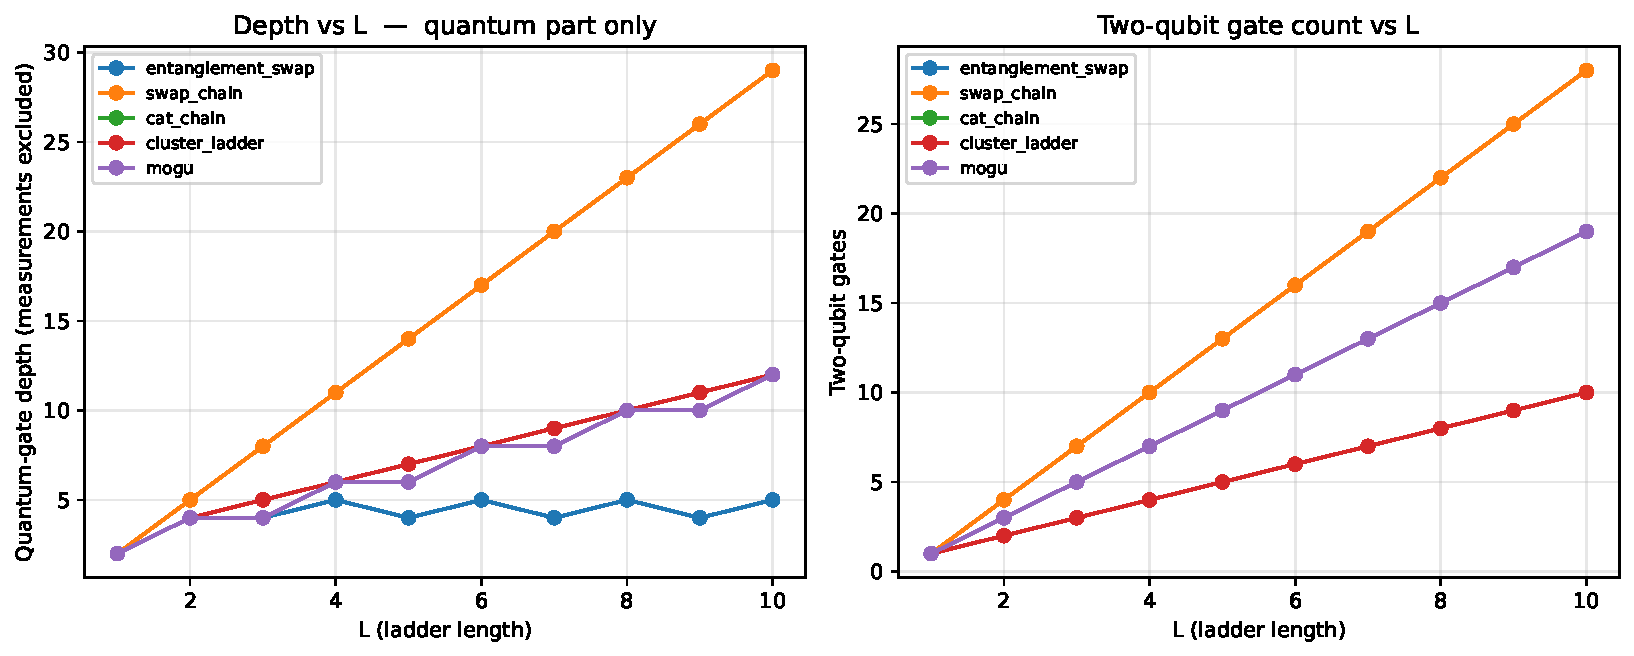
\includegraphics[width=0.96\textwidth]{figures/scaling_quantum.pdf}
  \end{center}
  \vspace{-0.3em}
  \footnotesize
  \textbf{What you see.} Protocol~I (\textcolor{e0col}{blue}) is the
  \alert{only depth-$O(1)$ curve} — its quantum part stays at $\leq 5$ layers
  for every $L$. Measurements and feed-forward Paulis are excluded from this
  count (they execute in classical real time). MOGU is linear with the smallest
  slope among the unitary protocols; SWAP-chain dominates both axes.
\end{frame}

% ============================================================
% Slide 11 — Benchmark noise
% ============================================================
\begin{frame}{Benchmark: Bell fidelity under depolarising noise}
  \begin{columns}[T,onlytextwidth]
    \begin{column}{0.62\textwidth}
      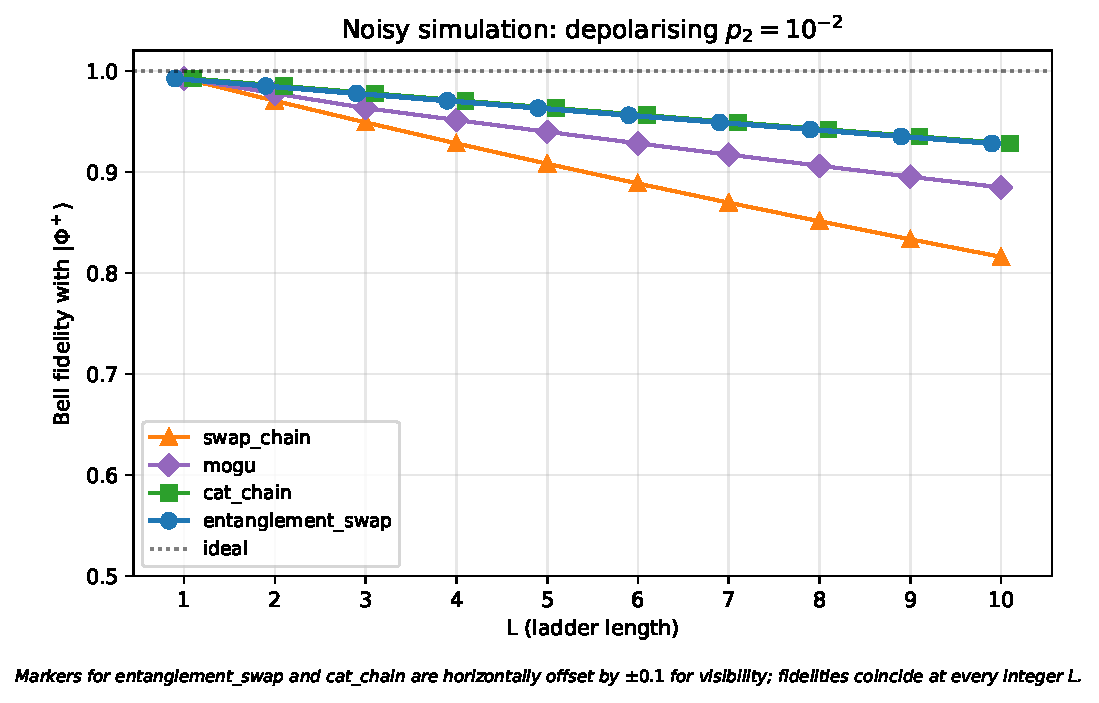
\includegraphics[width=\linewidth]{figures/noise_slides.pdf}
    \end{column}
    \begin{column}{0.38\textwidth}
      \footnotesize
      Symmetric two-qubit depolarising error $p_2=10^{-2}$ on every CNOT.
      \medskip

      \textbf{At $L=10$:}
      \begin{itemize}\setlength{\itemsep}{0.15em}
        \item Protocol~I: \alert{$0.928$}
        \item cat\_chain: $0.928$ \;{\scriptsize(same 2Q-gate count)}
        \item MOGU: $0.885$
        \item swap\_chain: $0.816$
      \end{itemize}

      \medskip
      Protocol~I (\textbf{$\bullet$}) and cat\_chain (\textbf{$\blacksquare$})
      give \emph{identical} fidelities at every $L$ — both incur $\approx N$
      noisy CNOTs touching $(e_0, e_1)$. The markers are jittered by
      $\pm 0.1$ in $L$ purely for visibility.
    \end{column}
  \end{columns}
\end{frame}

% ============================================================
% Slide 12 — When to use which
% ============================================================
% \begin{frame}{When to prefer which protocol}
%   \centering\footnotesize
%   \begin{tabular}{lll}
%     \toprule
%     \textbf{Hardware regime} & \textbf{Best choice} & \textbf{Why} \\
%     \midrule
%     Mid-circuit measurement + feed-forward & Protocol~I & $O(1)$ depth \\
%     Unitary-only                           & MOGU       & saturates LR bound \\
%     Small $L$, deep noise budget           & cat\_chain & fewest gates per endpoint \\
%     \bottomrule
%   \end{tabular}

%   \vspace{0.6em}
%   \begin{itemize}\footnotesize\setlength{\itemsep}{0.15em}
%     \item Both protocols verified to fidelity $>1-10^{-9}$ via \texttt{stim}
%           Clifford and Qiskit \texttt{Statevector} for $L\le 10$;
%           spot checks at $L\in\{20,30,50\}$.
%     \item \textbf{132 automated tests}, all passing.
%     \item Single codebase under \texttt{analysis/}.
%   \end{itemize}
% \end{frame}

% ============================================================
% Slide 13 — Thanks / references
% ============================================================
\begin{frame}[allowframebreaks]{References \& Summary}
  \textbf{Take-home}
  \begin{itemize}
    \item We proposed two protocols.
    \item Protocol~I: $O(1)$ depth, classical feed-forward.
    \item Protocol~II (MOGU): $L+2$ depth, measurement-free, depth-optimal for unitary 1D.
  \end{itemize}

  \medskip
  \textbf{Key references}
  \begin{itemize}\footnotesize
    \item Żukowski, Zeilinger, Horne, Ekert,
          \emph{Phys. Rev. Lett.}~\textbf{71}, 4287 (1993) — entanglement swapping primitive.
    \item Briegel, Dür, Cirac, Zoller,
          \emph{Phys. Rev. Lett.}~\textbf{81}, 5932 (1998) — quantum repeater.
    \item Bäumer~\textit{et al.},
          \emph{PRX Quantum}~\textbf{5}, 030339 (2024), arXiv:2308.13065 —
          long-range CNOT teleportation on 101 IBM qubits.
    \item Song~\textit{et al.},
          \emph{Phys. Rev. Applied}~\textbf{24}, 024068 (2025), arXiv:2409.06989 —
          constant-depth fan-out with feedforward.
  \end{itemize}

  \medskip
  \centering\Large Thank you. \\[0.3em]
  \small Questions?
\end{frame}

\end{document}
